\documentclass[12pt]{article}
 
\usepackage[margin=1in]{geometry} 
\usepackage{amsmath,amsthm,amssymb}
\usepackage{tikz}
\usepackage[linguistics]{forest}
\usepackage{booktabs}
% \usepackage{parskip}% http://ctan.org/pkg/parskip
% \usepackage{pgfplots}
\usepackage{amsmath}
\usepackage{setspace}
\usepackage{indentfirst}
\usepackage[linguistics]{forest}
\usepackage{graphicx}

% \usepackage[utf8]{inputenc}
\usepackage[english]{babel}

\theoremstyle{plain}
\newtheorem{theorem}{Theorem}
\newtheorem{corollary}{Corollary}[theorem]
\newtheorem{lemma}[theorem]{Lemma}

\usetikzlibrary{arrows,automata,positioning}

\pagenumbering{arabic}

\newcommand{\N}{\mathbb{N}}
\newcommand{\Z}{\mathbb{Z}}

% \let\pgfmathMod=\pgfmathmod\relax

% \newenvironment{theorem}[2][Theorem]{\begin{trivlist}
% \item[\hskip \labelsep {\bfseries #1}\hskip \labelsep {\bfseries #2.}]}{\end{trivlist}}
% % \newenvironment{lemma}[2][Lemma]{\begin{trivlist}
% % \item[\hskip \labelsep {\bfseries #1}\hskip \labelsep {\bfseries #2.}]}{\end{trivlist}}
% \newenvironment{exercise}[2][Exercise]{\begin{trivlist}
% \item[\hskip \labelsep {\bfseries #1}\hskip \labelsep {\bfseries #2.}]}{\end{trivlist}}
% \newenvironment{problem}[2][Problem]{\begin{trivlist}
% \item[\hskip \labelsep {\bfseries #1}\hskip \labelsep {\bfseries #2.}]}{\end{trivlist}}
% \newenvironment{question}[2][Question]{\begin{trivlist}
% \item[\hskip \labelsep {\bfseries #1}\hskip \labelsep {\bfseries #2.}]}{\end{trivlist}}
% \newenvironment{corollary}[2][Corollary]{\begin{trivlist}
% \item[\hskip \labelsep {\bfseries #1}\hskip \labelsep {\bfseries #2.}]}{\end{trivlist}}

% \newtheorem{lemma}[theorem]{Lemma}

\newenvironment{solution}{\begin{proof}[Solution]}{\end{proof}}

% \renewcommand{\thesubsubsection}{\alph{subsubsection})}
\makeatletter
\renewcommand{\p@subsubsection}{\thesubsection.\protect\eatbracket}
\makeatother
\def\eatbracket#1#2{#1\ifx)#2\else#2\fi}

\setlength{\parindent}{1cm} % Default is 15pt.
\doublespacing

\begin{document}
 
% \title{Final Paper}
% \author{Suzanne Wang \\ 
% Econ 350} 
% \maketitle

\begin{titlepage}
  \centering
  {\scshape\LARGE Wellesley College \par}
  \vspace{1cm}
  {\scshape\Large Economics Independent Study final paper\par}
  \vspace{3cm}
  {\huge\bfseries Models of Kidnap for Ransom Insurance\par}
  \vspace{2.5cm}
  {\Large Suzanne Wang\par}
%   \vfill
  supervised by\par
    {\large Casey Rothschild\par}

  \vfill

% Bottom of the page
  {\large Fall 2017\par}
\end{titlepage}

\section{Introduction}

Kidnapping for ransom is common in many developing countries. In recent years, annual recorded ransom payments have totaled over \$1.5 billion globally (Catlins, 2012). Seen now as a necessary cost of doing business, most large companies purchase kidnap for ransom insurance to cover their staff working in high risk areas (Economist, 2013). These insurance plans cover ransom payment to criminal kidnappers and hiring of consultants and negotiators, among other associated costs (). Recent research shows that kidnapping insurance is organized under a single governing body, Lloyd's of London, which enables firms to internalize the externalities from poorly managed insurance (Shortland, 2016). While research has examined game-theoretical models of kidnapping and insurance, kidnapping insurance has not been explored theoretically in a context of the unique private governance structure that is the Lloyd's market. We address this gap in the literature.

In media coverage of kidnaps for ransom, acts of terrorism and piracy are often the most visible. Terrorist kidnappings are not insurable, and many countries have no concessions policies which make it illegal to pay ransoms to terrorists. Terrorist kidnaps are often highly public, with million dollar ransoms and clear threats of violence. Though countries such as the UK, US, and Canada forbid paying terrorists (), ransoms are still often paid by the victim's family or myopic governments without no-concessions policies. Paying ransoms fund future terrorist activity, resulting in significant externalities. Indeed, research shows that between 2001-2013, negotiation successes with terrorist kidnappers increased kidnappings by 64-87\% by those groups (Brandt et al., 2016). [TODO: insert research about ineffectiveness of no-concessions policies] 

Piracy, another highly visible example of kidnapping for ransom, has also resulted in significant spillover effects. Unlike terrorist kidnappings, maritime piracy can be covered by insurance. While ransom levels were in the thousands in the early 2000s, piracy ransoms in Somalia skyrocketed to the millions in subsequent years, reaching a high of \$12 million in 2011 (De Groot et al., 2012). The high prices also contributed to an increase in frequency: Oceans Beyond Piracy estimates that Somali piracy cost about \$1.7 billion in 2016, while the World Bank estimates that it costs around \$18 billion to the economy when factoring costs such as changing shipping routes and paying high insurance premiums (World Bank, 2013). Like with terrorists kidnappings, knowledge surrounding the successful kidnaps and premium ransoms quickly spreads through the criminal community, leading to more groups to enter the market with high expectations. As a result of such high costs, many insurers suffered heavy losses, and some withdrew from the market entirely (World Bank, 2013), while other insurers sought naval protection and higher security from third parties (Shortland 2015). Though the economic cost of piracy has decreased in recent years (Oceans Beyond Piracy), the lack of price discipline has maintained a consistent frequency. []

Unlike terrorists and pirates, land-based criminal kidnaps are both insurable and reasonably stable in ransom quantity and price. While ransoms are often perceived to be vast amounts of money demanded alongside violent threats, that is hardly the case overall when looking at criminal kidnaps, which comprise 80\% of total kidnappings globally (Shortland 2016). Ransom amounts rarely exceed six-figures, much less \$1 million, generally hovering in the thousands or tens of thousands (Catlins 2012). According to Control Risks, a business risk consultancy retained by insurers, the median ransom in Nigeria out of 200 cases between 2006-2014 was less than \$5,500 (Control Risks 2015). Between 2000 and 2014, the rate of death for hostages was 0.5\%, caused most often by pre-existing medical conditions or rescue and escape attempts. According to multiple interviews, murder is highly unusual (Shortland, 2017). [TODO: insert concluding sentence?]

This striking relative stability of criminal kidnappings is a result of having a competitive market of insurers under one governing body. [TODO: insert footnote about how kidnappings are underreported] Recent research has shown that there is just a single source of kidnap insurance globally: Lloyd's of London (Shortland, 2016). While the market appears to be highly competitive, with about 20 insurers competing for business, they are all connected to Lloyd's in some way. Lloyd's is not an insurance company, but an insurance market where members join together as syndicates. For example, brokers and coverholders act on behalf of potential customers and work with underwriters in the Lloyd's Underwriting Room to obtain quotes. Each syndicate's underwriters price the risk and decide what will be covered. Members of Lloyd's provide capital, which Lloyd's holds in trust. These firms operated based on strict rules, that set Lloyd's as a governing body. The information sharing within Lloyd's provides huge value to its syndicates, and is crucial for business. Each syndicate has 1-2 kidnap specialists who develop deep knowledge in a ``boy-to-man'' profession. Since the underwriters are physically congregated in an underwriting room, syndicates can share information in passing and over lunch (Shortland, 2017). However, information sharing is extremely limited outside of Lloyd's (Guardian, 2014). Membership in Lloyd's is renewed each year, and Lloyd's can close any syndicate that acts against the market's interest. As a result, the syndicates adopt consistent practices that do not jeopardize their membership in Lloyd's (Stringham, 2015). Like in organized crime, where non-cooperation yields high risk of violence (Leeson, 2011), non-cooperation in Lloyd's results in a high risk of suffering losses from being excluded from the market.

[lloyd's infographic]

As seen with terrorist and pirate kidnappings, externalities from poorly-managed negotiations include high ransoms, which in turn encourage more kidnappers to enter the market with high payout expectations (De Groot et al., 2010). These externalities affect both social welfare as well as insurers, who are priced out of the market when they cannot cover high ransom costs nor sell insurance with adequately high premia. Insurers of kidnap for ransom are thus motivated to internalize these externalities. They do so by preventing moral hazard and lowering ransom costs. They stipulate that the clients must first raise the ransom payment amount themselves, then receive reimbursement after payment (Shortland, 2016). Furthermore, insurers often provide training to their clients on how to minimize risk in target countries, and perform security checks in their covered areas of operation (Business Insurance, 2008). Insurers also control knowledge of insurance coverage by forbidding client firms from discussing insurance with their employees (Marsh, 2011). By taking these steps to prevent moral hazard, insurers minimize the probability of kidnap. Another way to minimize this likelihood is to decrease ransoms. This is done through expert negotiators and consultants at crisis response companies hired by the insurer. In the event of kidnap, experienced negotiators advise the victim stakeholder on how to negotiate. They ensure that the client does not settle too early and too high, especially when they are cash-rich and willing, and despite the evidence showing that it results in a faster release, lower negotiation costs, and lower risks for the hostage (Ambrus et al., 2014). Ultimately, maintaining a low ransom equilibrium is of the utmost importance, to prevent a vicious cycle of more kidnappers entering the market, higher ransom expectations and demands, and if paid, a continued increase in kidnapping (Shortland 2016, UN 2013, Wright 2009). The result would be lower social welfare and insurers being priced out of the market. 

This paper focuses in on negotiation-- specifically its duration and quality. If negotiations are too long in an effort to maximally decrease a ransom, kidnappers respond with threats of and actual violence, as ``myopic insurers could cut short ransom negotiations to save themselves time, hassle, and cost [of hiring consultants] and reimburse high ransoms without 'punishment''' (Shortland, 2016). However, membership in Lloyd's prevents this. Professional negotiators can remain incredibly patient and spend weeks and months leveling with kidnappers, especially when the kidnappers' expectations are high. 

In addition to qualitative research, kidnapping and insurance have also been examined in a game theoretical framework. Selten (1977) modeled a 2-player game between a kidnapper and victim's family, showing that kidnapping is rational only when the kidnapper has a high willingness to kill, but not exceeding a certain threshold. Crettez and Deloche (2009) builds on Selten's model, capuring the kidnapping for non-monetary ransoms in the context of assasination of prominent political figures. Lapan and Sandler (1988) model kidnapping between the kidnapper and government instead, showing a multiperiod sequential game that includes reputational effects for the government, which influences terrorists' views on their willingness to grant future concessions. In examining when the government should pre-commit to not negotiating, they find that not negotiating should generally be avoided, which is consistent with empirical studies [TODO: add more about this?]. Fink and Pringle (2014) build upon these previous papers to include kidnap for ransom insurance, and explore under what conditions insurance should be purchased. In a 2 player game between a kidnapper and the victim's family, they find that a risk-averse family benefits from ransom insurance while most kidnappers do not benefit from it. They also show that increasing `successful' kidnappings increase the likelihood of kidnap, which makes insurance both more expensive and less attractive. Therefore, insurance companies should use divert some of their resources to risk reduction efforts, as they clearly do in the real world.

This paper seeks to build upon the recent game theoretic and political science research around kidnap for ransom insurance. We model a game between an insurer and its customer (a firm or family), showing cases both with and without the Lloyd's market. In the former, individual insurance firms within Lloyd's are aware that they are influencing the average negotiation (and therefore ransom levels), and cooperate negotiate at a set, average level. Firms that are not under a private governance structure, on the other hand, are not setting the private level of negotiation to equal the average, and are instead taking that environmental level as given and optimizing with only themselves in mind. We show that consumer welfare is maximized in a Lloyd's setting.

\section{The Model}

We model kidnapping as a two person game between the insurer and the firm, who purchases insurance for its employees. At the first stage, the insurer competes in a perfectly competitive market and price their premia, which also set their level of service through negotiation. The firm decides whether or not to purchase insurance and at what level. Then there are two moves by nature: a firm's employee is kidnapped with probability $p$, and if kidnapped, killed with probability $q$. We assume:
\begin{align*}
\begin{forest}
  [\textbf{Insurers}
    [][] [\textbf{Consumer} [] []
          [\textbf{Nature} 
          [\textbf{Nature}, edge label={node[midway,left,font=\scriptsize]{Client kidnapped with probability $p$}} 
              [{$(W-P-K)$}, edge label={node[midway,left,font=\scriptsize]{Client not killed with probability $1-q$}}] 
              [{$(W-P-D)$}, edge label={node[midway,right,font=\scriptsize]{Client killed with probability $q$}}]
          ],edge label={node[midway,left,font=\scriptsize]{Purchases insurance with premium $P$}} 
          [{$(W-P)$}, edge label={node[midway,right,font=\scriptsize]{Client not kidnapped with probability $1-p$}}
          ]
      ] [] [,edge label={node[midway,right,font=\scriptsize]{Chooses $N$ and associated $P(N)$}}]
    ] [] [,edge label={node[midway,right,font=\scriptsize]{Compete in market to price premium schedule $P(N)$}}]
  ]
\end{forest}
\end{align*}

Under a competitive market without Lloyd's, given a schedule of premia $P(N)$, consumers choose the level of negotiation $N$ that they desire, contributing to the average level of negotiation $\bar{N}$. Under Lloyd's, $N$ is a fixed value where $N = \bar{N}$ and insurers compete to price premia given that level of $N$.

The insurer's premium $P(p, R)$ is a function the probability of being kidnapped $p$ and the ransom level $R$. The probability of kidnap $p(\bar{N})$ is a function of the average level of negotiation by other insurers in the market, $\bar{N}$, as quick and easy negotiations motivate more kidnappings (Shortland, 2016). The ransom $R(N, \bar{N})$, paid out by insurers to kidnappers, is a function of how much insurers negotiate, as well as the average level of negotiation by other insurers in the market.\footnote{$N$ is the individual level of negotiation, which represents the effort and resources the insurer is willing to put into extracting a hostage, and $\bar{N}$ is the environmental level of negotiation, which represents the average amount insurers in the market negotiate.} At the time of pricing their premia, insurance companies decide on a set level of negotiation $N$, which in turn decide their premium $P(p(\bar{N}), R(N, \bar{N}))$.

The firm begins with initial wealth $W$, and pays the premium $P$ when purchasing insurance. In the case of kidnapping, the firm suffers a cost $K$. In the case of death, they suffer cost a $D$. The firm's employee faces a probability of death $q(N)$, which is a function of $N$, or how hard the insurer negotiates. 

The firm has von Neumann-Morgenstern preferences with expected utility $EU$ in this game given the 3 possible outcomes--- not kidnapped, kidnapped and freed, and kidnapped and killed:
\begin{align*}
EU = (1-p)U(W-P) + p(1-q)U(W-P-K) + pqU(W-P-D)
\end{align*}

\subsection{Assumptions}

Premium, $P(p(\bar{N}), R(N, \bar{N}))$, is a function of probability of kidnap and ransom. Assume that $\frac{\partial P}{\partial R} > 0$ and $\frac{\partial P}{\partial p} > 0$, since premia go up along with ransom amounts and probability of kidnap. We assume that higher individual and environmental levels of negotiation drive ransoms down, so $\frac{\partial R}{\partial \bar{N}} < 0$ and $\frac{\partial R}{\partial N} < 0$. We also assume that $\frac{\partial p}{\partial \bar{N}} \leq 0$, since higher environmental levels of negotiation dissuade criminals from kidnapping. 

Given that premium is a function of $p$ and $R$, both functions of $\bar{N}$, we can assume that $\frac{\partial P}{\partial \bar{N}} = \frac{\partial p}{\partial \bar{N}} + \frac{\partial R}{\partial \bar{N}}$. Since both $\frac{\partial p}{\partial \bar{N}}$ and $\frac{\partial R}{\partial \bar{N}}$ are less than $0$, $\frac{\partial P}{\partial \bar{N}} < 0$. In other words, a higher average level of negotiation results in a lower premium, as both kidnap probability and ransom levels decrease.

Probability of death, $q(N, \bar{N})$ is a function of individual and environmental negotiation levels $\bar{N}$. Assume that higher average negotiations imply that kidnappers are able to tolerate higher levels of individual negotiation, so the probability of death decreases. Thus $\frac{\partial q}{\partial \bar{N}} < 0$. However, $\frac{\partial q}{\partial N} > 0$, since negotiating harder and longer on an individual level results in a higher risk of death.

Finally, we assume that an increase in the premium, probability of kidnapping, or probability of death result in a lower expected utility for the firm, so $\frac{\partial EU}{\partial P} < 0, \frac{\partial EU}{\partial p} < 0$, and $\frac{\partial EU}{\partial q} < 0$.

\subsection{Competitive Equilibrium}

With each negotiation, insurers contribute to the average level of negotiation in a particular area, which in turn influences ransom levels $R$. Due to information sharing between criminals, previous levels of ransom and negotiation influence the desirability of engaging in kidnapping. Quick and easy negotiations and high payouts compel more kidnappers to enter the market with higher expectations for ransom. On the other hand, long and strenuous negotiations with low payouts can maintain a more stable ransom level and low frequencies of kidnapping. In this model, $\bar{N}$ captures these externalities: ransom $R$ is determined not only by an individual insurer's negotiation but the environmental levels as well. If the precedent for negotiation $\bar{N}$ is low, where insurers are willing to settle early and pay higher ransoms, kidnappers enter negotiations with higher expectations and would be unwilling to settle for a lower amount than if previous victim stakeholders had negotiated harder for lower ransoms. On the other hand, if the average levels of negotiation are high, kidnappers anticipate a more arduous ransom negotiation process, thus decreasing ransom expectations in addition to their likelihood of kidnapping.

Taking $\bar{N}$ as given, the consumer problem is then:
\begin{align*}
\underset{N}{max}EU(N, \bar{N}) = \underset{N}{max}&(1-p(\bar{N}))U(W-P(p(\bar{N}), R(N, \bar{N}))) \\
&+ p(\bar{N})(1-q(N, \bar{N}))U(W-P(p(\bar{N}), R(N, \bar{N}))-K) \\
&+ p(\bar{N})q(N, \bar{N})U(W-P(p(\bar{N}), R(N, \bar{N}))-D)
\end{align*}

For a given $\bar{N}$, consumers choose a premium that reflects their individual rational level of negotiation, $N^*(\bar{N})$. In competitive equilibrium, $\bar{N} = N$. We are therefore looking for an $\bar{N}$ so that when consumers solve this problem, the $N$ consumers choose is equal to the original $\bar{N}$, such that the market is in equilibrium and the consumers are solving their own optimization problem. At equilibrium, the actual $\bar{N}$ is equal to expectations. For any other set of expectations of $\bar{N}$, the actual behavior will not be consistent with those expectations. When making choices about $N$, consumers are predicting what $\bar{N}$ is going to be. In equilibrium, consumer expectation is correct. The solution to this problem is characterized by a first order condition at equilibrium where $\frac{\partial EU(\bar{N}^*, \bar{N}^*)}{\partial N} = 0$. We assume in competitive equilibrium, $N>0$ and $N=0$ is not optimum.

\subsection{Lloyd's Problem}

In a private governance structure, the Lloyd's market chooses a uniform level of negotiation, facilitating cooperation on $N$. Insurers who do not reach a certain standard of negotiation risk getting kicked out of the market, losing access to an essential web of information, the Lloyd's brand, and its "chain of security" fund structure (). Incentivized to follow the Lloyd's standard, insurers set their private $N$ to equal the market standard. By collectively choosing the same $N$, the environmental level of negotiation equals the private level: $N = \bar{N}$. The maximization problem is therefore:
\begin{align*}
\underset{N, \bar{N}}{max} (1-p)U(W-P) + p(1-q)U(W-P-K) + pqU(W-P-D) \qquad s.t. \; N = \bar{N}
\end{align*}

\section{Analysis}

\subsection{Lloyd's Market Equilibrium} 

\noindent
The following proposition characterizes the equilibrium under Lloyd's. 

\bigskip
\noindent
\textbf{Proposition 1.} Let $\bar{N}^*$ denote the competitive equilibrium. Starting at the competitive equilibrium, it is welfare-improving to increase $N$, so $\frac{d}{dN}EU(N,\bar{N}(N))_{\bar{N}^*} > 0$ when $\bar{N}(N)\equiv N$.

\bigskip

\noindent
Before turning to the proof, we prove the following lemma:

\begin{lemma}
$\frac{\partial EU}{\partial \bar{N}} > 0$
\end{lemma}

\begin{proof}
Observe that $\frac{\partial EU}{\partial \bar{N}} = \frac{\partial F}{\partial P} \frac{\partial P}{\partial \bar{N}} + \frac{\partial F}{\partial p} \frac{\partial p}{\partial \bar{N}} + \frac{\partial F}{\partial q} \frac{\partial q}{\partial \bar{N}}$. By assumption, $\frac{\partial F}{\partial P} < 0, \frac{\partial F}{\partial p} < 0, and \frac{\partial F}{\partial q} < 0$, and $\frac{\partial P}{\partial \bar{N}} <0, \frac{\partial p}{\partial \bar{N}} < 0, \frac{\partial q}{\partial \bar{N}} < 0$. As a result, all terms in  $\frac{\partial EU}{\partial \bar{N}}$ are positive, which makes $\frac{\partial EU}{\partial \bar{N}} > 0$.
\end{proof}

\noindent
\textbf{Proof of Proposition 1:}

\begin{proof}
Observe that $\frac{d}{dN}EU(N,\bar{N}(N))_{\bar{N}^*} = \frac{\partial EU(\bar{N}^*, \bar{N}^*)}{\partial N} + \frac{\partial EU}{\partial \bar{N}}$. By the first order conditions from the competitive problem, the first term is 0. By Lemma 1, the second term is positive. 
\end{proof}

\subsection{Example of Competitive Equilibrium}

Proposition 1 shows that starting at the competitive equilibrium, it is welfare-improving to increase N. In other words, the Lloyd's market enforces a higher N that results in a higher expected utility. To better illustrate this, we construct an example generated in Python.

We use the von Neumann Morgenstern expected utility function and the following functional forms:
\begin{align*}
U(x) &= \sqrt[]{x} \\
p(\bar{N}) &= \frac{10}{\bar{N} + 10} \\
q(N, \bar{N}) &= ln(\frac{N}{150} + \frac{10}{\bar{N}}) \\
R(N, \bar{N}) &= \frac{2000}{N + 1} + \frac{10000}{\bar{N} + 1} + 2000 \\
P(p(\bar{N}), R(N,\bar{N})) &= pR 
\end{align*}

\subsubsection{Competitive Equilibrium}

In the competitive market, the consumer faces a schedule of premia from insurers and takes $\bar{N}$ as given. The consumer chooses the level of negotiation $N$ in response that prices their premium $P(p(\bar{N}), R(N,\bar{N}))$ to maximize expected utility. The following figure depicts the consumer's rational level of negotiation $N^*$ for any given $\bar{N}$.

\begin{figure}[h]
\centering
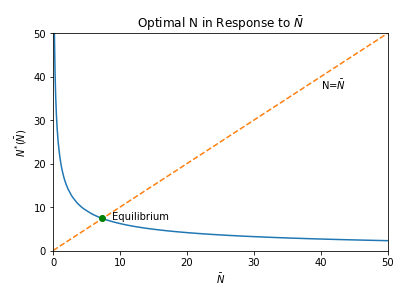
\includegraphics[width=13cm]{competitive.png}
\end{figure}

At equilibrium, $N^*(\bar{N}) = \bar{N}$. The intersection of the curve and 45-degree dotted line reveal the equilibrium point, where $N=7.37$ in this example. At negotiation levels less than 7.37, consumers would choose an $N$ such that $N > \bar{N}$. At $\bar{N} > 7.37$, however, the level of $N^*(\bar{N})$ that maximizes expected utility is less than $\bar{N}$. This suggests that if the average level of negotiation appears to be high, consumers can choose lower individual levels.

We can also observe the level of expected utility the corresponds to this point, where the consumer takes $\bar{N} = 7.37$ as given.

\begin{figure}[h]
\centering
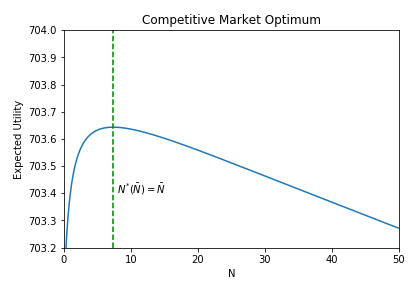
\includegraphics[width=13cm]{comp_eu.png}
\end{figure}

\newpage
At the maximum point where $\frac{\partial EU(\bar{N}^*, \bar{N}^*)}{\partial N} = 0$, $N^*(\bar{N})=7.37$, which equals $\bar{N}$. At this equilibrium, the behavior of individual firms is rational and the environment is consistent with their behavior.

\subsubsection{Lloyd's Equilibrium}

Under the Lloyd's market, it is always the case that $N = \bar{N}$, as the governing body sets the standards for negotiation. Therefore, insurers price their premium exactly where $N = \bar{N}$, and consumers choose whether or not to purchase insurance. Using this example, we can find the value $N$ that maximizes expected utility.

\begin{figure}[h]
\centering
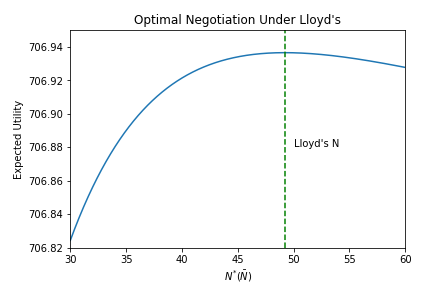
\includegraphics[width=10cm]{lloyds2.png}
\end{figure}

\newpage
Under Lloyd's, the rational level of negotiation is $49.21$. Zooming out, we can observe the optimal $N$ under competitive equilibrium relative to Lloyd's. 

\begin{figure}[h]
\centering
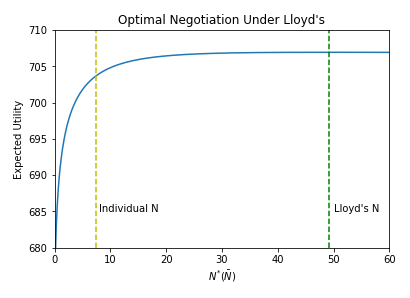
\includegraphics[width=10cm]{lloyds1.png}
\end{figure}

This is a clear representation of Proposition 1. Given $\bar{N}(N)\equiv N$, at the individual rational $N$ the slope of expected utility is positive. It is thus welfare-improving to increase $N$--- higher negotiation levels under Lloyd's internalize externalities, resulting in higher expected utilities.

\section{Discussion}

This paper has examined the kidnapping and ransom insurance market under both a competitive market and single governing body, Lloyd's of London. We highlight the role of negotiation on both the individual and environmental levels in each case. The average environmental levels of negotiation $\bar{N}$ capture externalities associated with kidnapping and ransom insurance: for any given area, having a quick and easy average level of negotiation (i.e. a lower $\bar{N}$) result in a higher likelihood of kidnapping $p$ along with higher levels of ransom $R$ and possibility of death $q$. At competitive equilibrium, consumers take the environmental level of negotiation $\bar{N}$ as given, and choose their own negotiation level $N$ to reflect their expectations for $\bar{N}$, such that $N=\bar{N}$. At the Lloyd's equilibrium, $\bar{N}$ is determined by Lloyd's, and insurers set their $N$ to equal $\bar{N}$. Our analysis shows that at competitive equilibrium, consumers choose a lower level of $N$ that does not internalize the externalities associated with negotiation, whereas Lloyd's consumers subscribe to a level of $N$ that maximizes their expected utility.

Other features not captured in this model include addressing adverse selection and moral hazard. For example, insurers set different standards of training in their insurance contracts, to minimize moral hazard by customers who operate in high risk areas (Control Risks, 2010). Further extensions could also include applying a similar model to the context of terrorist kidnapping or piracy, incorporating the criminal as a player who "monitor" the effectiveness of negotiation and risk management measures (Shortland, 2017), or considering the impact of uninsured consumers in the market for more external validity.

Our results show that Lloyd's of London serves as a highly effective governing body in the kidnapping and ransom insurance market. It not only enables fluid information sharing and secure capital flow, but also internalizes externalities through setting standards for negotiation. Lloyd's succeeds in areas where actual governments fail, and improves both the welfare of its consumers and society as a whole.
\\

[TODO: import bibtex]


\end{document}
